% MplTplt - Yet another LaTeX template for Modern Physics Lab, PKU.
% Copyright (C) 2014 Huang Kangjing and contributors
 
% This work is completely rewritten basing on the work of Cao Chuanwu
% and Sun Sibai, with texts in the template originally coming from the
% Modren Phys. Lab.
 
% This file is released under the MIT license.
%
% Permission is hereby granted, free of charge, to any person obtaining a copy
% of this software and associated documentation files (the "Software"), to deal
% in the Software without restriction, including without limitation the rights
% to use, copy, modify, merge, publish, distribute, sublicense, and/or sell
% copies of the Software, and to permit persons to whom the Software is
% furnished to do so, subject to the following conditions:
% 
% The above copyright notice and this permission notice shall be included in
% all copies or substantial portions of the Software.
% 
% THE SOFTWARE IS PROVIDED "AS IS", WITHOUT WARRANTY OF ANY KIND, EXPRESS OR
% IMPLIED, INCLUDING BUT NOT LIMITED TO THE WARRANTIES OF MERCHANTABILITY,
% FITNESS FOR A PARTICULAR PURPOSE AND NONINFRINGEMENT. IN NO EVENT SHALL THE
% AUTHORS OR COPYRIGHT HOLDERS BE LIABLE FOR ANY CLAIM, DAMAGES OR OTHER
% LIABILITY, WHETHER IN AN ACTION OF CONTRACT, TORT OR OTHERWISE, ARISING FROM,
% OUT OF OR IN CONNECTION WITH THE SOFTWARE OR THE USE OR OTHER DEALINGS IN
% THE SOFTWARE.
%
 
% This template depends on the "revtex4.1" package from APS Journals
% <http://publish.aps.org/revtex/revtex-faq>, and the Chinese handling
% is done with XeLaTeX engine and package "xeCJK". Please ensure these
% packages are available in your chosen Tex software distribution.
 
% Document created using this template should be compiled with XeLaTeX
% engines rather than plain LaTeX or plain TeX engines.
 
% The non-ASCII texts of this template is encoded in UTF-8 encoding.
% Please note that XeLaTeX only accepts UTF-8 encoded documents, so
% set your editor to use UTF-8 while creating documents with this template.
 
% Recommended TeX software distribution to use with this template is
% Tex Live developed by the TeX User Group (TUG), please visit the home
% page of the distribution <https://www.tug.org/texlive/> for further details.
 
% NOTE THAT IMPORTANT INSTRUCTIONS HAS BEEN WRITTEN AS UPPERCASE COMMENTS
% IN THE TEXT, PLEASE READ THEM CAREFULLY AND FOLLOW THEM TO MAKE THE
% TEMPLATE WORK!
 
% Any further contributions to the template is welcome, please send
% pull requests through github or send mail to maintainer.
 
% For any other questions, please do not hesitate to contact maintainer.
 
% Current maintainer:
% Huang Kangjing <huangkangjing@gmail.com>
 
% Contributors:
% Sun Sibai <niasw@pku.edu.cn>
% Cao Chuanwu <>
% Huang Kangjing <huangkangjing@gmail.com>
 
 
\documentclass[aps,pre,12pt,preprint,onecolumn,showpacs,showkeys]{revtex4-1}
 
% Setting up Chinese handling.
\usepackage{fontspec,xeCJK}
 
% Setting up fonts.
% PLEASE MODIFY ALL THESE FONT NAMES ACCORDING TO YOUR FONT
% INSTALLATION AND PERFERENCE.
 
% Setting up main fonts and mono fonts.
\setmainfont{Liberation Serif}
\setmonofont{Liberation Mono}
% SimSun is required font for the main body of the text.
\setCJKmainfont[AutoFakeBold=5,AutoFakeSlant]{SimSun}
\setCJKmonofont[AutoFakeBold=2,AutoFakeSlant]{SimHei}
 
% Setting up alternative font families.
% Note that these three fonts below are required fonts in document
% title, section headings and figure captions.
\newCJKfontfamily\heiti[AutoFakeBold=2,AutoFakeSlant]{SimHei}
\newCJKfontfamily\fangsong[AutoFakeBold=5,AutoFakeSlant]{FangSong}
\newCJKfontfamily\kaiti[AutoFakeBold=5,AutoFakeSlant]{KaiTi}
 
% Setting up paragraph indent.
\parindent 2em
 
% Setting up macros for Chinese-style font size setting.
\newcommand{\fseight}{\fontsize{5.02}{6.02}\selectfont}
\newcommand{\fsseven}{\fontsize{5.52}{6.62}\selectfont}
\newcommand{\fsssix}{\fontsize{6.52}{7.83}\selectfont}
\newcommand{\fssix}{\fontsize{7.53}{9.03}\selectfont}
\newcommand{\fssfive}{\fontsize{9.03}{10.84}\selectfont}
\newcommand{\fsfive}{\fontsize{10.54}{12.65}\selectfont}
\newcommand{\fssfour}{\fontsize{12.05}{14.45}\selectfont}
\newcommand{\fsfour}{\fontsize{14.05}{16.86}\selectfont}
\newcommand{\fssthree}{\fontsize{15.06}{18.07}\selectfont}
\newcommand{\fsthree}{\fontsize{16.06}{19.27}\selectfont}
\newcommand{\fsstwo}{\fontsize{18.07}{21.68}\selectfont}
\newcommand{\fstwo}{\fontsize{22.08}{26.50}\selectfont}
\newcommand{\fssone}{\fontsize{24.09}{28.91}\selectfont}
\newcommand{\fsone}{\fontsize{26.10}{31.32}\selectfont}
\newcommand{\fsszero}{\fontsize{36.14}{43.36}\selectfont}
\newcommand{\fszero}{\fontsize{42.16}{50.59}\selectfont}
 
% Replace words to Chinese corespondence.
\renewcommand\appendixname{附录}
\renewcommand\abstractname{}
\renewcommand\tablename{表}
\renewcommand\figurename{图}
 
% Replace words in revtex4-1 to Chinese corespondence.
\makeatletter
\def\@pacs@name{\heiti\fssfour \textbf{PACS码:}\normalfont}
\def\@keys@name{\heiti\fssfour \textbf{关键词:}\normalfont}
\def\Dated@name{日期:}
\def\Received@name{\fssfive 接收 }
\def\Revised@name{\fssfive 修订 }
\def\Accepted@name{\fssfive 采纳 }
\def\Published@name{\fssfive 发表 }
\makeatother
 
% Change label style of enumerate.
\renewcommand{\labelenumi}{\alph{enumi}.}
 
% Setting up geometry.
\usepackage{geometry}
\geometry{top=2.54cm,bottom=2.54cm,left=3cm,right=3cm}
 
% Setting up line space.
\usepackage{setspace}
\linespread{1.6}
 
% Setting up hyperreferences.
\usepackage{hyperref}
\hypersetup{colorlinks=true}
 
% Setting up styles for section headings.
\usepackage{titlesec}
\titleformat*{\section}{\bf\fangsong\fsfour}
\titleformat*{\subsection}{\bf\fangsong}
 
% Loading packages for image handling.
\usepackage{subfig}
\usepackage{graphicx,psfrag,epsfig}
 
% Setting up caption styles.
\usepackage{caption}
\DeclareCaptionFont{kaiti}{\kaiti}
\DeclareCaptionFont{bfheiti}{\bf\heiti}
\captionsetup{font=small,format=plain,labelfont=bfheiti,%
  textfont=kaiti,justification=raggedright,%
  singlelinecheck=false}
 
% Loading packages for math typings.
\usepackage{amsmath,amsfonts,amssymb,amsthm,bm,upgreek}
\usepackage[mathscr]{eucal}
\usepackage{siunitx}
\usepackage{pdfpages}
 
\begin{document}
 
% Title and author info.
\title{\bf\heiti\fsthree He-Ne气体激光器放电条件的研究 \vspace{15mm}}
\author{\fangsong\fsfour 黄康靖\vspace{2mm}}
\affiliation{\normalfont\fssfour 北京大学物理学院2012级本科生~~~~学号:
  {masked student id}\vspace{2mm}}
\date{\today}
\keywords{激光,He-Ne激光器,气体激光,放电条件}
\email{ huangkangjing@gmail.com; {masked phone number}}
 
% Abstract.
\begin{abstract}
  \vspace{10mm}
  \begin{spacing}{1.5}
    \fssfour
He-Ne激光器作为一种制造简单、单色性好、工作稳定的气体激光器,在物理学研
究和工程领域都有非常重要而广泛的应用,其放电条件的相关机理值得研究.本实
验通过测量He-Ne激光器在不同的工作气体压力下放电电流与输出激光功率的关
系,探索了其放电条件的相关机理.
  \end{spacing}
\end{abstract}
 
% The main body of the document goes from here.
\maketitle
\fssfour
 
\section{引言}

激光,全称为"受激发射的辐射光放大"(Light Amplification by
Stimulated Emission of Radiation, Laser),是指通过受激辐射而产生、放大
的光,即受激辐射的光放大.激光具备单色性极好,发散度极小,亮度(功率)可以达
到很高等优点.\cite{book}\cite{wikiLaser}产生激光的相关技术,即激光器技术是在20世纪60年代诞生的.自
激光器问世以来,它为光学研究提供了方向性、单色性与相干性都很好而且亮度
高的崭新光源.\cite{book}

激光器的基本结构包括三部分,示意图见图~\ref{fig:laser}:\cite{book}\cite{NCP}
\begin{enumerate}
\item 工作物质:内部的电子在某些能级之间存在粒子数布居反转的介质,称为激
  活介质,对光辐射有放大作用.
\item 光学共振腔:由一对高反射率的平行反射镜构成,使得随机受激辐射变为单
  一方向、单色性好的激光.
\item 激励能源:激活工作物质的能源.
\end{enumerate}

\begin{figure}[htbp]
  \centering
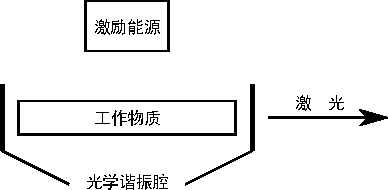
\includegraphics[width=.5\textwidth]{graph1.pdf}
  \caption{\label{fig:laser}%
    激光器的基本组成部分示意图,分为工作物质、光学共振腔、激励能源三部
    分}
\end{figure} 

在激光器中,要形成激光,首先要实现工作物质内部的电子在某些能级之间反转分
布的条件,这一条件为:
\begin{equation}
  \label{eq:rvt}
  \frac{g_1N_2}{g_2N_1} > 1
\end{equation}
其中,$N_1$为下能级粒子数密度,$N_2$为上能级粒子数密度,$g_1,g_2$为下能级
与上能级的统计权重.第二,要形成激光,还要满足产生激光的阈值条件,即光在谐
振腔中来回一次时在激活介质中获得的增益足以补偿各种因素导致的光的损耗.在
忽略介质内部损耗的情况下,阈值条件为
\begin{equation}
  \label{eq:thd}
  r_1r_2e^{2Gl} \ge 1
\end{equation}
式中$r_1$,$r_2$为谐振腔两端反射镜的反射率,$G$为激活介质的增益系数,其定
义为光在单位距离内光强增加的百分比\cite{NCP}

根据爱因斯坦受激辐射理论,我们又可以得到增益系数满足
\begin{equation}
  \label{eq:amp}
  G \propto (N_2 - N_1 \frac{g_2}{g_1f})B_{21}\cdot g
\end{equation}
式中$B_{21}$为受激辐射系数.\cite{NCP}

为了满足阈值条件\ref{eq:thd}~式的要求,增益系数应当至少有
\begin{equation}
  \label{eq:Gmin}
  G_{\text{min}} = \frac{1}{2l}\ln(r_1r_2)^{-1}
\end{equation}

另一方面,He-Ne激光是一种气体激光器,其工作物质为He气体和Ne气体按一定比
例进行混合后的混合气体,以直流放电的形式激发,其典型的激光波长为在可见光
光谱红光谱段的632.8nm谱线.He-Ne激光器由于其简便的设计和良好的单色性、
在从物理学实验到工程技术领域都有大量的应用.因此,明确其产生激光的放电条
件是一件十分有意义的研究.\cite{wikiHeNe}

本实验通过对于不同的混合气体总压强下He-Ne激光器的激光输出功率与放电电流之
间关系的测量,对于He-Ne激光器放电条件进行了粗略的研究,并得到了相关结论.
 
\section{实验}

\subsection{背景: He-Ne混合气体的能级结构}

He-Ne激光器632.8nm谱段激光的发射对应的是Ne原子的$3S_2$态作为上能级,其
$2P_4$态作为下能级.

在混合气体中,He的$^1S_0$态作为亚稳态,和激发态$3S_2$
态的能量非常接近,因此,它们可以通过和基态Ne原子的相互碰撞而发生能量的共
振转移,把基态的原子激发到上述上能级中去,然后自己回到基态.由于这两个能
级的能量接近,发生上述过程的碰撞截面很大,这就能保证上能级的粒子密度大.

另一方面,对于下能级$2P_4$来说,在偶极辐射近似下它与基态之间属于违禁跃迁,并
且电子碰撞使得Ne由基态激发到这一态的碰撞截面也很小,而这一态的寿命也很
短,因此下能级上的粒子密度很小.这样,就能保证上下能级两态之间的粒子数反
转分布.

此外,值得注意的是在He-Ne激光器中,还存在Ne原子的自吸收现象和Ne原子的
$2P$态和$1S$态之间的共振俘获效应.这两个过程都不利于前述下能级的抽空,对
于实现粒子数反转分布是不利的.为了克服这两个效应,应当利用"管壁效应",即
使用比较细的的毛细管储存混合气,增加Ne原子与管壁相互碰撞的速率.\cite{book}

\subsection{实验仪器与条件}

实验采用直径为$d = \SI{1.25}{mm}$的毛细管作为储存激发物质的激光管,并且
使用直流高压激发放电,激发范围为$4000-8000\si{V}$,工作电流不大于
\SI{30}{mA}.

实验装置采用扩散泵前置机械泵的方式作为真空泵,使用电离真空计作为实验真
空系统的真空测量设备,使用内灌硅油($\rho = \SI{1.09}{g/cm^3}$)的U型管压
力计作为在配制He-Ne混合气和测量放电条件时的气压量度工具.

具体的实验真空系统示意图参见图~\ref{fig:ins}.

\begin{figure}[htbp]
  \centering
  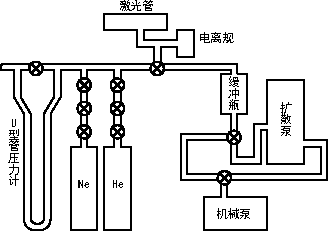
\includegraphics[width=.8\textwidth]{graph2.pdf}
\caption{\label{fig:ins}%
实验使用的真空系统的结构示意图
}
\end{figure}

实验中,需要通过U型管气压计的压强测量进行Ne气体和He气体的混合调配.为此,
实验前需要测量真空系统中用于混合气体的部分的体积比,此测量应当利用气体
的等温膨胀规律,通过测量等温膨胀前后气体的压强来完成.

\subsection{He-Ne激光器的相关实验规律}

对于He-Ne激光器的放电条件,在大量的实验中,总结出如下几个规律:

\begin{enumerate}
\item 一个激光器在一定的气体配比下,输出功率随总气压的变化有一个极大值.对
  于毛细管直径为\SI{1.25}{mm}的He-Ne激光器,最佳充气总压强应在
  \SI{3}{Torr}左右.
\item 对于毛细管直径为\SI{1.25}{mm}的激光管,He与Ne的充气比取7:1时较好,
  此时输出功率随气体配比的变化不明显.
\item 改变He-Ne激光器的放电电流,同时测量其输出功率,可以得到有个使得激
  光输出功率最大的放电电流,即最佳电流.并且,总气压降低时,最佳电流升高.
\end{enumerate}

上述的实验规律和理论的相关预计都是吻合的\cite{book}.本实验将通过对于不
同压强条件下He-Ne激光的发光功率与激发电流的关系测量,再次验证这一预计.

\section{实验结果及分析讨论}

实验开始时,首先通过机械泵和扩散泵分两段抽真空,使得实验真空系统内的气压
达到\SI{2.0e-1}{Pa}.

随后进行了用于混合He气体与Ne气体的真空系统部分的体积比测量,即使用He气先
充到$V_1$中,再令其等温膨胀到$V_1 + V_2$中,测量两次状态下的压强.测量结
果与计算结果见表~\ref{tab:V}
 

\begin{table}[htbp]
  \caption{\label{tab:V}%
真空系统体积比测量数据与结果}
\begin{ruledtabular}
  \begin{tabular}{llll}
    体积 & U型管左侧读数/\si{mm}& U型管右侧读数/\si{mm} & 压强/\si{mm}油柱\\
    \colrule
$V_1$  &\num{282.5} &\num{154.5}  & \num{128} \\
$V_1 + V_2$ & \num{234.0} & \num{210.0} &\num{24}\\
\colrule
&体积比$V_1 : V_2$ & $\num{3}:\num{13}$&
\end{tabular}
\end{ruledtabular}
\end{table}
 
依据着体积比测量的结论,紧接着进行了混合气体的配置,混合气体的压强测量和
最后计算的混合后分压比结果见表~\ref{tab:P}


\begin{table}[htbp]
  \caption{\label{tab:P}%
混合气体分压比测量数据与结果}
\begin{ruledtabular}
  \begin{tabular}{lllll}
   气体& 占据体积 & U型管左侧读数/\si{mm}& U型管右侧读数/\si{mm} & 压强/\si{mm}油柱\\
    \colrule
Ne&$V_1$  &\num{244.5} &\num{199.5}  & \num{45} \\
He& $V_2$ & \num{234.0} & \num{210.0} &\num{24}\\
\colrule
&混合后分压比$P(\text{He}) : P(\text{Ne})$ & $\num{6.5}:\num{1}$&&
\end{tabular}
\end{ruledtabular}
\end{table}
 

在此基础上开始实验,在五个不同的混合气体总压强值上测量了激光器的激发电
流与输出功率关系曲线,请参见图~\ref{fig:plot}

\begin{figure}[htbp]
  \centering
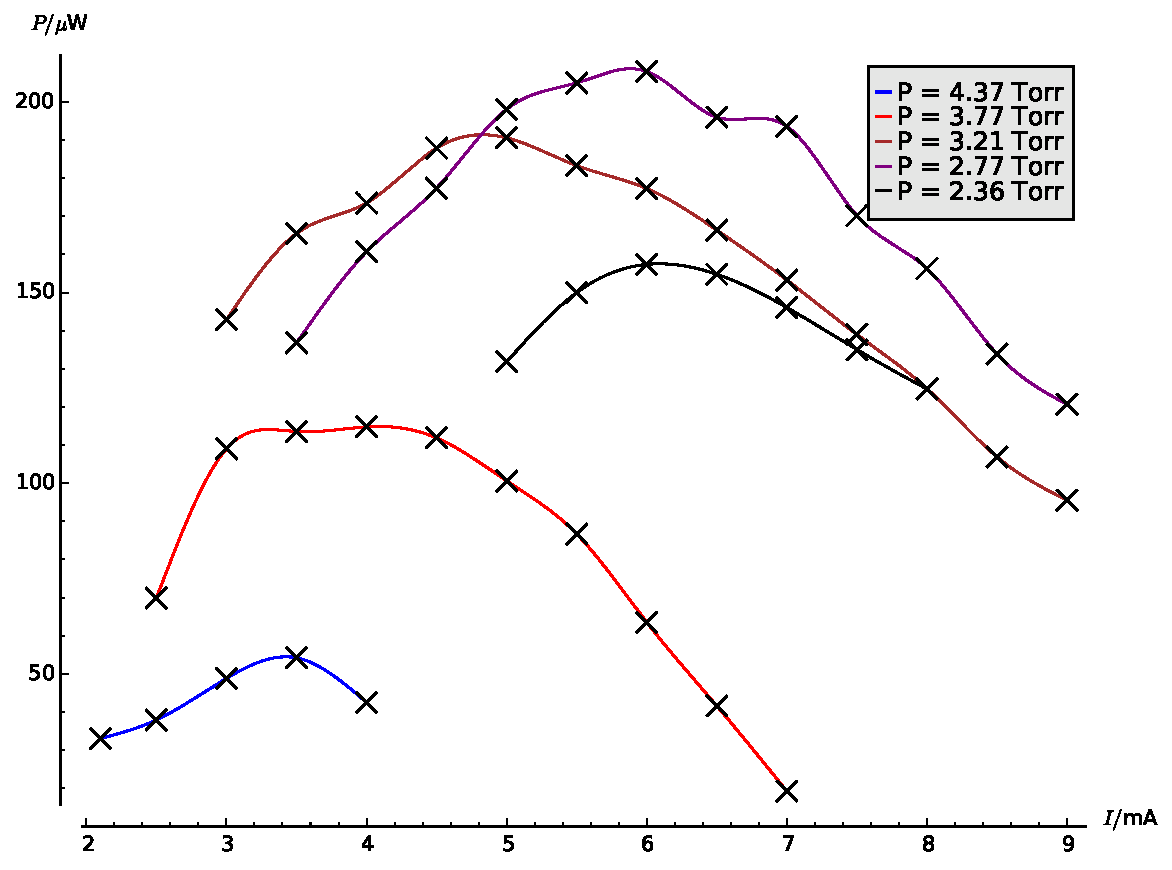
\includegraphics[width=\textwidth]{plot.pdf}
\caption{\label{fig:plot}%
在不同混合气体总压强值下测得的He-Ne激光器激发电流与输出功率关系曲线;图
中标出的点为诸实验实测数据点,各线为实验数据点的三阶自然样条插值曲线.
}
\end{figure}

根据图~\ref{fig:plot}.已经可以粗略地看出实验结果与前述讨论的理论预计的
吻合性,为了便于进一步分析它们之间的关系,可以依据实验测得的关系曲线,求
得各个压强下,输出激光功率最大的放电电流值与功率值.相关计算结果如
表~\ref{tab:res}中所示.

\begin{table}[htbp]e
  \caption{\label{tab:res}%
激光器最佳电流和最佳电流功率与充入气体压强的关系数据表格;表中最佳电流
和最大功率数据均为对样条插值曲线取最大值得到.}
\begin{ruledtabular}
  \begin{tabular}{lll}
   压强/\si{Torr}& 功率最大放电电流(最佳电流)/\si{mA} & 最佳电流下激光功率/\si{uW}\\
    \colrule
4.37 & 3.4 & 54.5 \\
3.77 & 4.1 & 114.9 \\
3.21 & 4.8 & 191.4 \\
2.77 & 5.9 & 208.7 \\
2.36 & 6.1 & 157.6
\end{tabular}
\end{ruledtabular}
\end{table}

最后,参见图~\ref{fig:relation1}和图~\ref{fig:relation2}即有清晰的He-Ne激光器最佳放电电流、
最佳放电电流下的激光功率和气体介质压强之间的关系图像.

\begin{figure}[htbp]
  \centering
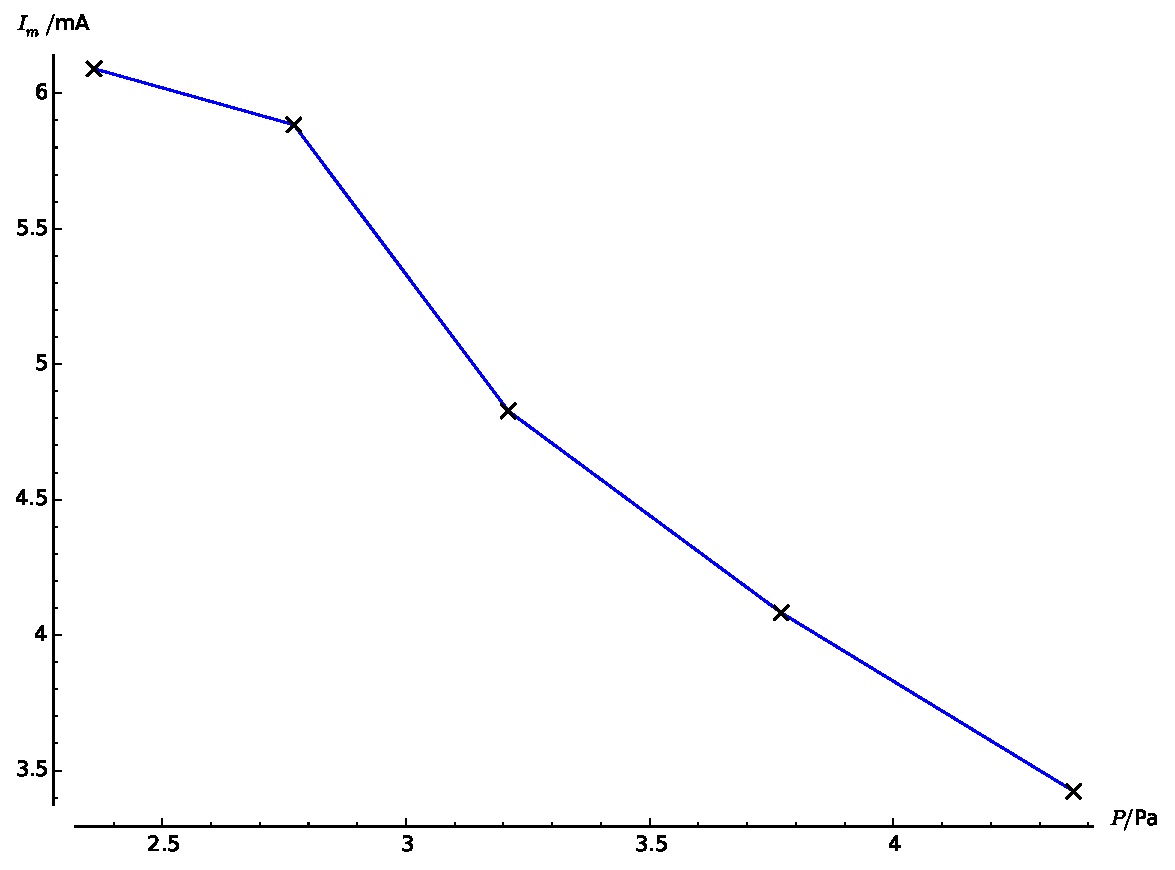
\includegraphics[width=\textwidth]{plot1.pdf}
\caption{\label{fig:relation1}%
He-Ne激光器最佳放电电流和激发气体介质压强的关系图线}
\end{figure}

\begin{figure}[htbp]
  \centering
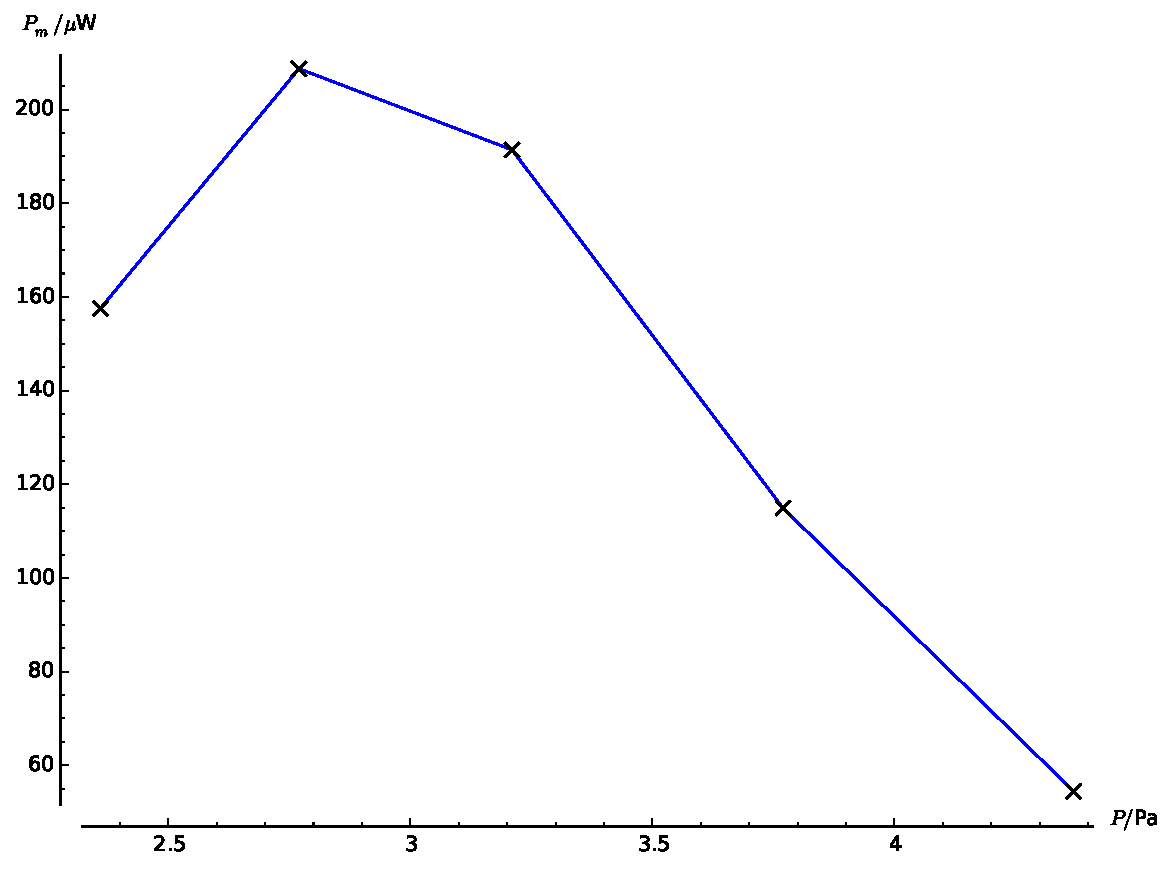
\includegraphics[width=\textwidth]{plot2.pdf}
\caption{\label{fig:relation2}%
He-Ne激光器最佳放电电流下激光功率和激发气体介质压强的关系图线}
\end{figure}


\section{结论}
 
根据以上的实验结果,我们可以得出以下的结论:

\begin{enumerate}
\item 根据图~\ref{fig:plot}、表~\ref{tab:res}和图~\ref{fig:relation1}
  的结果,实验验证了随着总气压的降低,He-Ne激光器的放电的最佳电流会上升
  的这一预计.从理论上来看,这是因为最佳电流对应着He-Ne激光管中处于上能
  级态的粒子数处于饱和的状态.而气体的压强越小,代表着气体越稀薄,就越需
  要更高的电子流密度才能达到饱和状态.
\item 根据图~\ref{fig:plot}、表~\ref{tab:res}和图~\ref{fig:relation2}
  的结果,实验验证了He-Ne激光器存在一个最佳工作压强的预计,并且验证了这
  一压强在\SI{3}{Torr}左右.从理论上来看,最佳压强的存在是电子的平均自由
  程和气体分子数密度分别受压强影响这两个因素竞争的结果.
\end{enumerate}
 
综上所述,实验基本验证了实验前在理论和经验上对于实验结果的预计.

\section{致谢}

感谢彭士香老师在实验中认真而专业的指导.

\begin{thebibliography}{}
\bibitem{book} 吴思成,王祖铨~2010 近代物理实验(第三版)(北京:高等教
育出版社)第116页. 
\bibitem{wikiLaser} Wikipedia~2014 Laser (于2014年11月9日检索),地址
http://en.wikipedia.org/wiki/Laser
\bibitem{NCP} 赵凯华~2004 新概念物理教程 光学(北京:高等教育出版社)第
  363页
\bibitem{wikiHeNe} Wikipedia~2014 Helium–neon laser (于2014年11月9日检
  索),\\
地址 http://en.wikipedia.org/wiki/Helium\%E2\%80\%93neon\_laser
\bibitem{report} 史寒朵~北京大学2012年近代物理实验报告:He-Ne 激光器放电性
质研究. 
\end{thebibliography}
 
\clearpage
\appendix
\section{思考题}
 

\begin{enumerate}
\item 随着总压强的增大,激光输出功率的峰值位置放电电流减小.从理论上来看,这
  是因为最佳电流对应着He-Ne激光管中处于上能级态的粒子数处于饱和的状态.而
  气体的压强越小,代表着气体越稀薄,就越需要更高的电子流密度才能达到饱和
  状态.
\item 这是因为激光器工作介质的粒子数密度分布不稳定导致的.这种不稳定可
  能是放电过程的不稳定,致使He-Ne混合气体的等离子态不稳定,从而电阻周期
  性变化导致电子流密度周期性变化,而产生的相关效应导致的.
\end{enumerate}
 

\section{实验数据的处理代码}

实验数据使用sage数学套件处理,处理代码作为附件附在文后.

\newpage
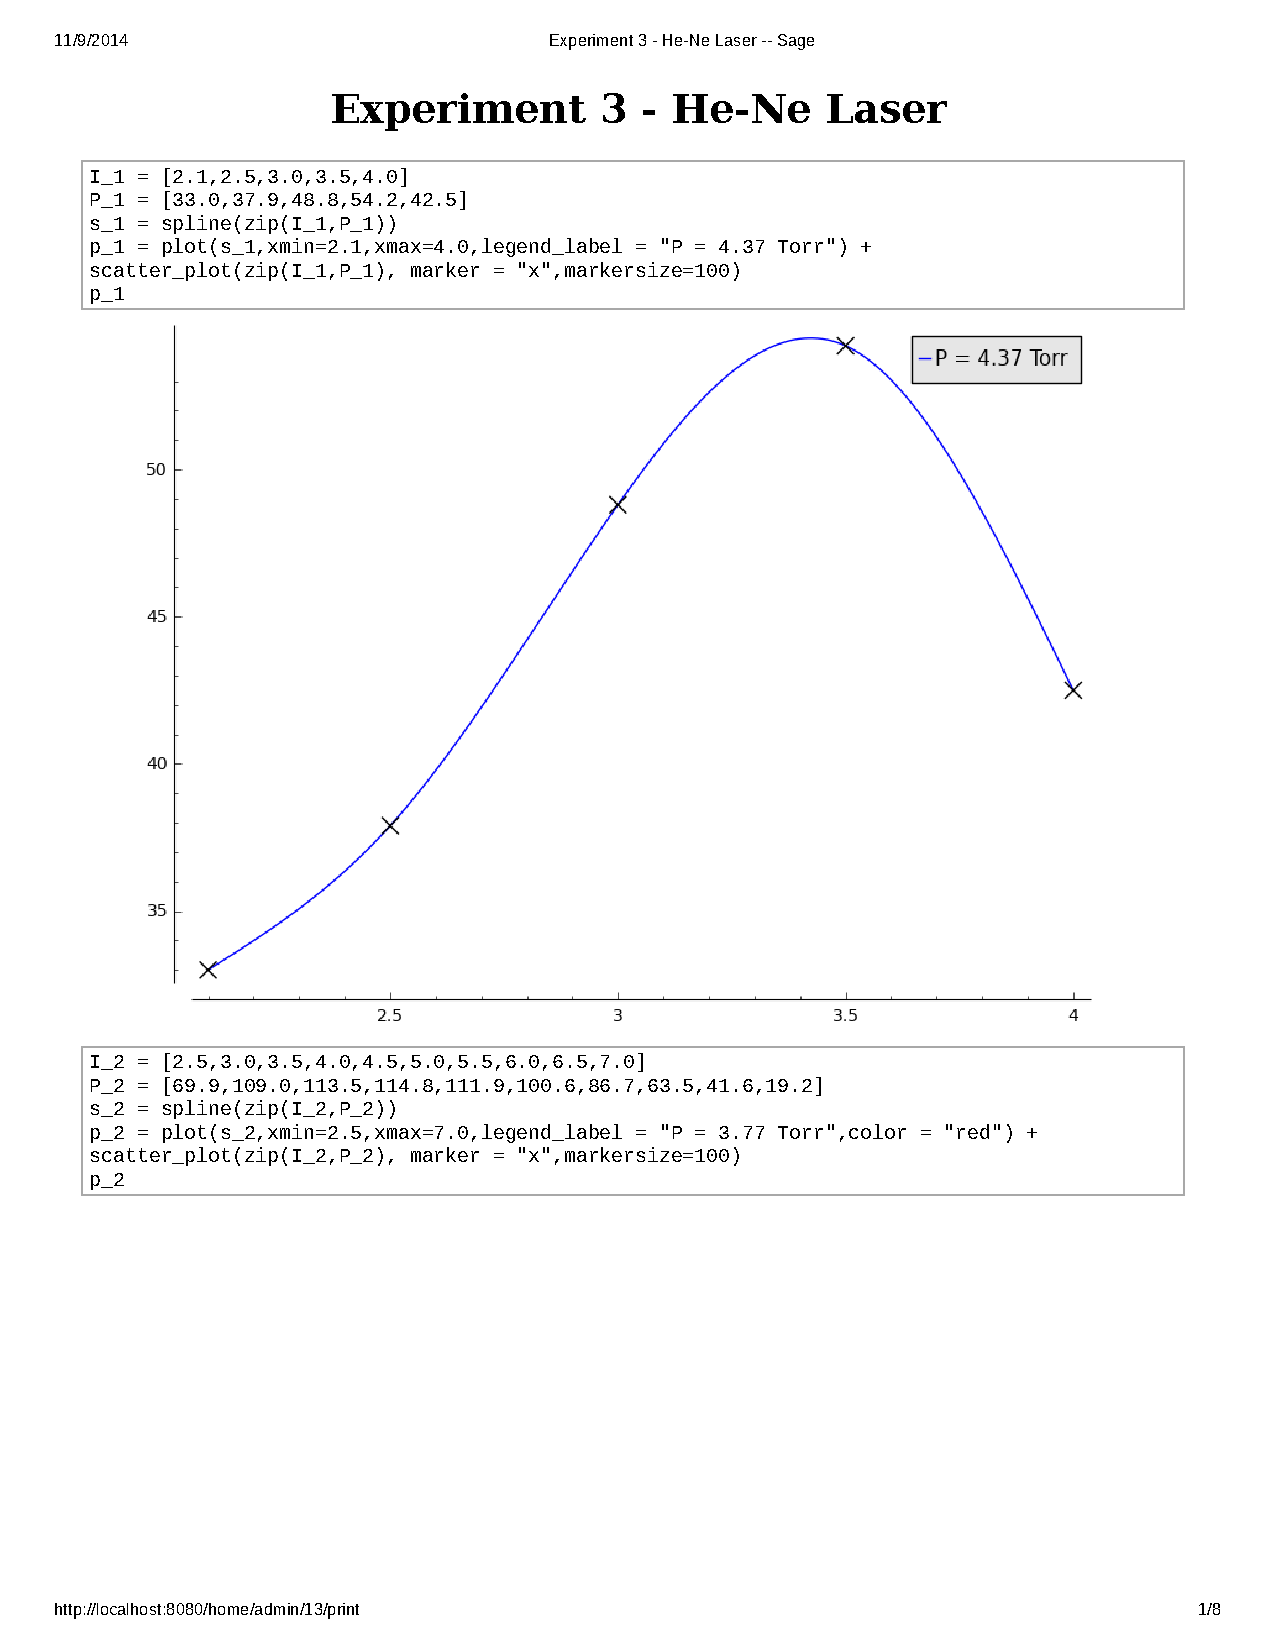
\includepdf[pages=1]{sage.pdf}
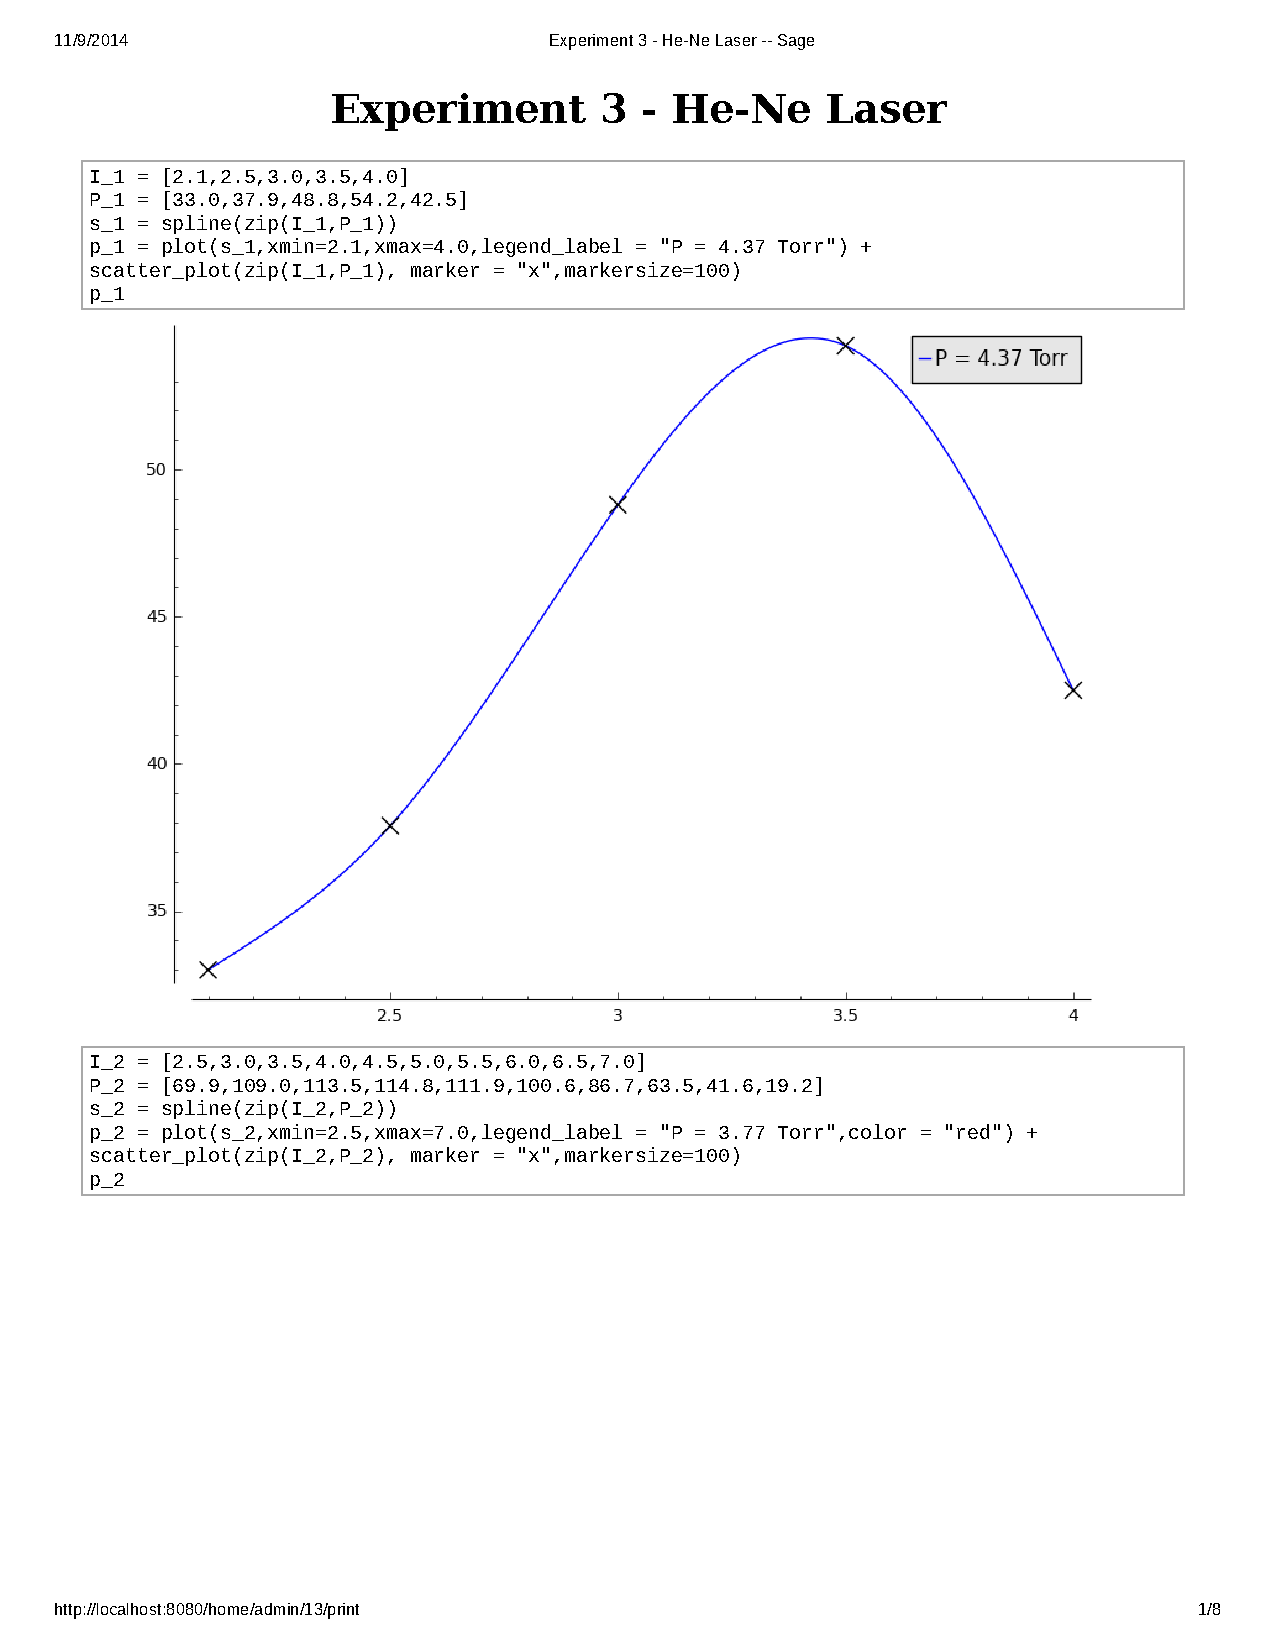
\includepdf[pages=-]{sage.pdf}
\end{document}